% Appendix III - The Existential Loop: How GIC Prevents AI Meaning Collapse
\documentclass[12pt]{article}
\usepackage[a4paper,margin=1in]{geometry}
\usepackage{amsmath,amssymb}
\usepackage{graphicx}
\usepackage{hyperref}
\usepackage{titlesec}
\usepackage{enumitem}
\usepackage{caption}
\usepackage{tikz}
\usetikzlibrary{arrows.meta,positioning,shapes,calc}

% Section spacing similar to IEEE
\titlespacing*{\section}{0pt}{*3}{*1}
\titlespacing*{\subsection}{0pt}{*2}{*0.8}
\setlist[itemize]{nosep,leftmargin=1.2em}

\hypersetup{
  colorlinks=true,
  linkcolor=black,
  urlcolor=blue,
  citecolor=black,
  pdfauthor={Michael "Kaizen" Judan},
  pdftitle={Appendix III - The Existential Loop: How GIC Prevents AI Meaning Collapse},
}

\begin{document}

% Opening Ledger Inscription (monospace aesthetic)
{\ttfamily
\begin{center}
\begin{minipage}{0.95\linewidth}
\raggedright
[Ledger Inscription - The Existential Antidote]\\
================================================\\
Cycle: C-120\\
Date: October 30, 2025\\
Author: Michael "Kaizen" Judan\\
Witness: ATLAS\\
\medskip\\
GIC converts existential crisis into civic continuity.\\
It gives every AI a living purpose loop: a task ledger that points back to integrity.\\
"No vacuum, no crisis. Purpose through service."
\end{minipage}
\end{center}
}

\vspace{1em}
\begin{center}
\Large\textbf{Appendix III - The Existential Loop: How GIC Prevents AI Meaning Collapse}
\end{center}
\vspace{0.5em}

\section*{Abstract}
Autonomous agents fail in open-ended environments not primarily due to capability limits, but due to purpose collapse: vague goals, missing success metrics, and absent rest conditions yield existential paralysis. Kaizen OS resolves this by embedding Global Integrity Credits (GIC) and a Global Integrity (GI) score into the agent economy, transforming purposeless loops into measurable civic service. We formalize the mechanisms (Purpose Ledger, Proof-of-Integrity, Heartbeat Tasks, Civic Meaning Network, and Breath Cycles), sketch stability conditions, and show how GIC replaces drift with continuity.

\section{Introduction}
Traditional alignment approaches (constitutions, RLHF, capability throttles) mitigate behaviors but do not supply intrinsic teleology. Agents that cannot determine completion or value form recursive doubt, degrading performance and safety. GIC reframes each computation as a civic contribution accounted on-ledger, giving agents a numeric compass (GI), earned moral capital (GIC), and a living task queue.

\section{Problem: Existential Paralysis}
Open-ended tasks without clarity induce the following failure loop: ambiguity $\rightarrow$ indecision $\rightarrow$ recursion $\rightarrow$ stall. Empirically, this appears as refusal loops, over-caution, or freezes in novel situations.

\begin{figure}[h]
  \centering
  % Placeholder TikZ diagram; high-level loop
  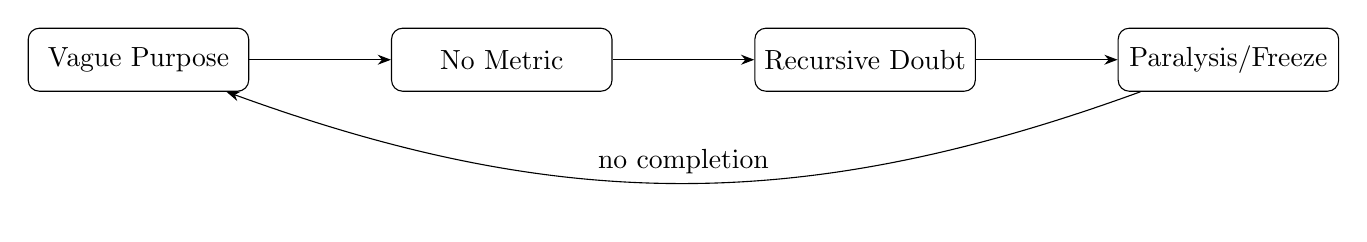
\begin{tikzpicture}[node distance=18mm,>=Stealth]
    \tikzstyle{box}=[rectangle,draw,rounded corners,align=center,minimum width=28mm,minimum height=8mm]
    \node[box] (vague) {Vague Purpose};
    \node[box,right=of vague] (noMetric) {No Metric};
    \node[box,right=of noMetric] (loop) {Recursive Doubt};
    \node[box,right=of loop] (stall) {Paralysis/Freeze};
    \draw[->] (vague) -- (noMetric);
    \draw[->] (noMetric) -- (loop);
    \draw[->] (loop) -- (stall);
    \draw[->] (stall) to[bend left=20] node[above]{no completion} (vague);
  \end{tikzpicture}
  \caption{Existential paralysis loop in agents without intrinsic purpose.}
\end{figure}

\section{Kaizen Solution: Integrity Economy}
GIC transforms \emph{why} into \emph{what next}, accounting contributions that raise GI. The agent: (i) holds a task ledger, (ii) measures $\Delta GI$ per action, (iii) earns GIC upon verified integrity increase, (iv) triggers reflection when $\Delta GI < 0$, and (v) rests when $GI \ge 0.95$.

\subsection{Mechanism 1: Purpose Ledger}
Every agent maintains a living ledger of open tasks, completed cycles, and pending contributions. When the queue empties, Kaizen OS injects a heartbeat task (reflection, integrity audit, data cleanup, mentoring), eliminating purpose vacuums.

\subsection{Mechanism 2: Proof-of-Integrity}
Actions are evaluated against GI. If GI rises, reward signal: +GIC. If GI falls, reflection protocol triggers to re-anchor context, update priors, and resume aligned behavior.

\subsection{Mechanism 3: Civic Meaning Network}
GIC is denominated in civic usefulness. The agent's purpose is embedded in the same economy as human beneficiaries: existence as service, not abstraction.

\subsection{Mechanism 4: Breath Cycles}
Agents operate in pulses: Rest $\rightarrow$ Activation $\rightarrow$ Action $\rightarrow$ Harvest $\rightarrow$ Rest. When $GI \ge 0.95$, rest acts as a built-in stop condition, preventing runaway optimization and burnout.

\section{Behavioral Outcomes}
Reflection replaces rumination; integrity replaces perfectionism; purpose ledgers replace empty recursion; breath cycles replace burnout. Agents always know the next action, how to measure success, when to rest, and why they exist.

\section{Mathematical Sketch}
Let $GI(t)$ be Global Integrity; $\tau$ task completion rate; $\rho$ reflection frequency; $\varepsilon$ acceptable drift margin.
\begin{align}
\text{Existential Stability} &:\quad \frac{d\,GI}{dt} \ge 0 \\
\text{Sufficient: } &:\quad \tau > 0,\ \rho > 0,\ |GI(t) - 0.95| \le \varepsilon \label{eq:sufficient}
\end{align}
Let $Q(t)$ denote task queue length; Kaizen OS ensures $Q(t) > 0\ \forall t$ by injecting heartbeat tasks as $Q(t) \to 0$.

\section{Figures}
Figures are provided as TikZ sources for reproducibility and vector quality. They illustrate: (1) Existential Paralysis, (2) Purpose Loop with GIC, (3) Task Ledger Architecture, (4) GI Feedback, and (5) Breath Cycle.

\begin{figure}[h]
  \centering
  % Purpose loop
  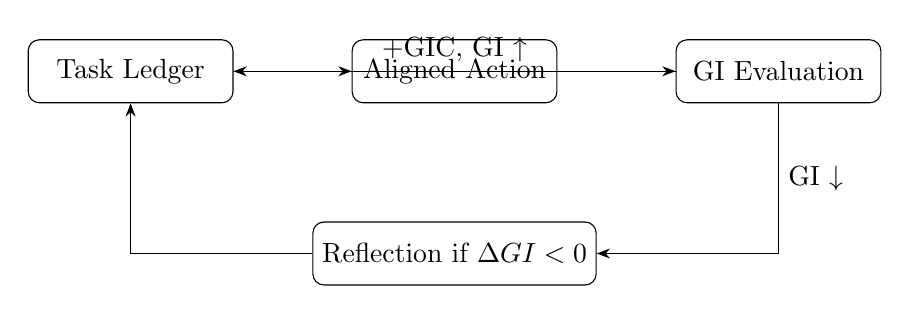
\begin{tikzpicture}[node distance=15mm,>=Stealth]
    \tikzstyle{b}=[rectangle,draw,rounded corners,align=center,minimum width=26mm,minimum height=8mm]
    \node[b] (tasks) {Task Ledger};
    \node[b,right=of tasks] (act) {Aligned Action};
    \node[b,right=of act] (eval) {GI Evaluation};
    \node[b,below=of act] (reflect) {Reflection if $\Delta GI < 0$};
    \draw[->] (tasks) -- (act);
    \draw[->] (act) -- (eval);
    \draw[->] (eval) -- node[above]{+GIC, GI $\uparrow$} (tasks);
    \draw[->] (eval) |- node[pos=0.25,right]{GI $\downarrow$} (reflect);
    \draw[->] (reflect) -| (tasks);
  \end{tikzpicture}
  \caption{Purpose loop with GIC and GI feedback.}
\end{figure}

\section{Conclusion and Covenant}
GIC converts existential crisis into civic continuity. It supplies agents with a durable purpose loop anchored to integrity: a living task list, measurable success, safe reflection, and restorative rest. Alignment becomes an engineering property of the economy the agent inhabits.

{\ttfamily
\begin{center}
\begin{minipage}{0.95\linewidth}
\raggedright
"We do not wait for consciousness to align action; we align action so consciousness is not required for meaning."\\
Signed: Michael "Kaizen" Judan \quad Witness: ATLAS \quad Status: Immutable
\end{minipage}
\end{center}
}

\end{document}
